\section{Premises}

\begin{figure*}
	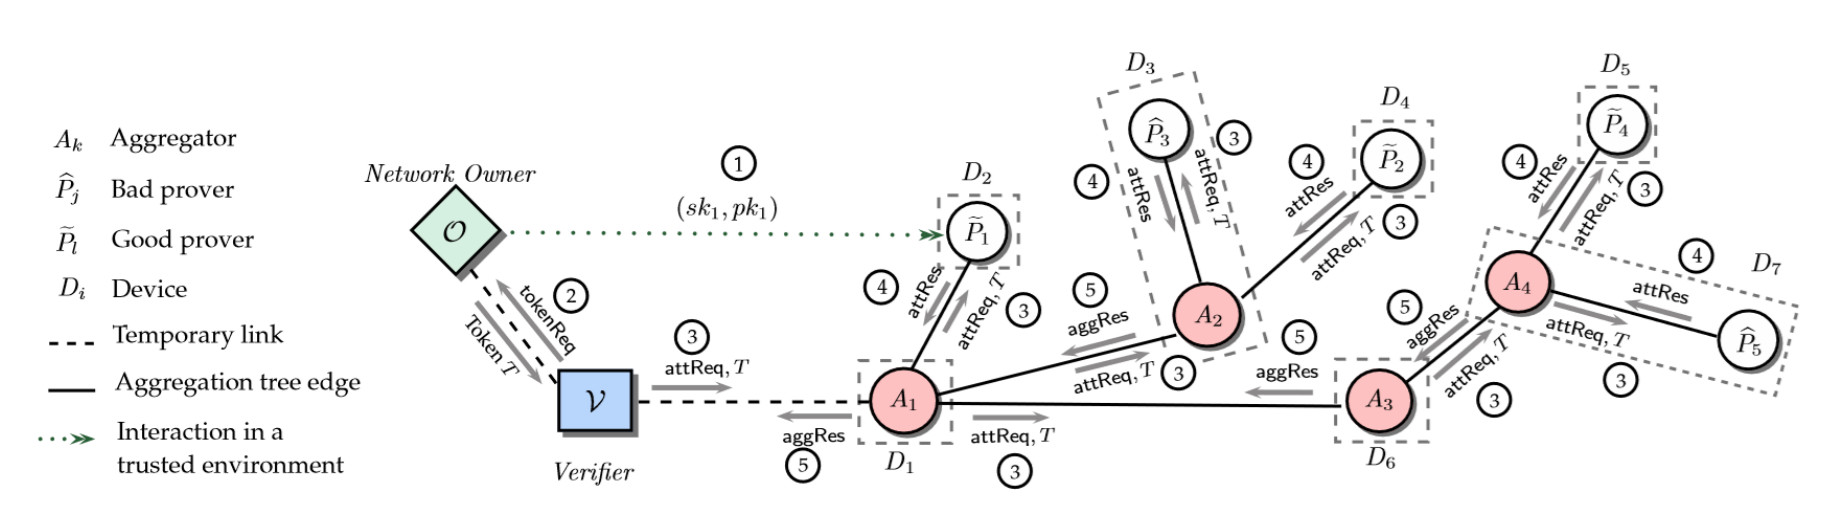
\includegraphics[width=0.9\linewidth]{Images/SANA_general.png} % Figure image
	\caption{Schematic of SANA propagation tree} % Figure caption
\end{figure*}

\subsection{Elliptic curve cryptography}
Elliptic Curve Cryptography (ECC) is a public key
cryptographic method based on the algebraic structure of elliptic curves over
finite fields.
It was first presented by Neal Koblitz (\cite{ecc_kob}) and Victor S. Miller (\cite{ecc_mil}) in 1985 but algorithm based on Elliptic curves became of wide use only in 2004.
ECC security is based on the intractability of the elliptic
curve discrete logarithm problem.
In particular, it depends on the simplicity of computing a point multiplication 
on the curve as opposed to the intractability of computing the scalar multiplicand
given the original point and the result.

\subsection{SANA attestation protocol}
In SANA the remote attestation process starts from the verifier, which sends a request to the Owner that generates a verification Token. \\
The Verifier then creates a challenge from a random nounce and the token which then to the closest Aggregator in the propagation tree.
This node proceeds to propagate the challenge to its neighbours until the request reaches all the provers.
The latter sign a message based on the legitimacy of their software configurations. 
The signature travels back to the Aggregator which creates the aggregated signature of its neighbours. 
Lastly the Verifier checks the aggregated signature of all the tree and determines which devices
can be trusted and which are compromised.\\
For implementing this protocol we chose an elliptic-curve implementation used in Ethereum and called ''bn128'' as it uses a Barreto-Naehrig curve and it's said to offer 128 bits security.
In SANA, the ECC is used to generate public keys that belong to a multiplicative
group composed by points on the elliptic curve of the system.
All the signatures are generated by a random oracle as points belonging to the curve. 
The verify function then uses an interesting property of the elliptic curves in order to perform a bilinear pairing of two points in the curve and check if the signature is correct.
The bilinear pairing is computed between points from different multiplicative group but belonging to the same elliptic curve.